\documentclass[11pt,letterpaper]{article}
\usepackage{graphicx, geometry, amsmath, hyperref, url, natbib, booktabs, longtable, xcolor, listings}
\geometry{margin=1in}
\hypersetup{colorlinks=true, linkcolor=black, citecolor=black, urlcolor=black}
\renewcommand{\topfraction}{0.9}
\renewcommand{\bottomfraction}{0.8}
\renewcommand{\textfraction}{0.07}
\renewcommand{\floatpagefraction}{0.75}

\title{Barometric Boiling Formula: Structural Error at 4000 m}
\author{}
\date{}

\begin{document}
\maketitle

\begin{abstract}
Simple barometric formulas are often used to estimate how the boiling point of water falls with altitude. What matters is how well they predict measured boiling points, and we could not test that: no measured boiling record with station pressure, elevation and thermometer uncertainty could be verified. We therefore report what can be tested against a reference. On a shared reference grid (0 to 4,000 m) coupled to the IAPWS industrial formulation saturation curve, the isothermal barometric form adds a structural error relative to the lapse-rate form of 0.588 K at 4,000 m, which is 0.088 K above a pre-set 0.5 K target. This is a single exploratory, reference-only screen: it has no interval and no measured data, and it bounds only the model's own structural error. The term grows with altitude. Whether the formula meets the 0.6 K total error budget against measured boiling points remains untested. A refitted Antoine equation has the lowest held-out error of three vapour-pressure routes, but that ranking is provisional.
\end{abstract}

\section{Introduction}\label{sec:intro}

The boiling point of water sets the temperature of cooking, sterilisation and many industrial steps, and it falls with altitude because the ambient pressure falls. Water boils at 373.12 K at sea level and several kelvin lower at 4000 m, and the exact drop depends on the pressure model used to estimate it. Barometric formulas, which map altitude to pressure, are the usual way to make that estimate without a local measurement. Their accuracy against measured boiling points determines whether they can be trusted for cooking guidance, instrument calibration and altitude-based corrections.

The gap is that a formula's accuracy against the reference saturation equation says little about its accuracy against measurement, and the two are often conflated. Measured boiling records carry station pressure, elevation and thermometer uncertainty, and few of them are published in a form that can be checked. We did not find enough of them to test the formula against measurement, so the gap stays open here.

Our idea is to separate the two sources of error. We decompose the difference between a barometric boiling estimate and the reference into a structural term, which comes from the barometric model itself, and a measurement term, which needs measured records. This paper reports the structural term and states what the measurement term would require.

Our contributions are as follows.

\begin{itemize}
  \item The headline: on a shared reference grid (0 to 4,000 m), the isothermal barometric structural term is 0.588 K at 4,000 m, 0.088 K above the 0.5 K structural target. This is an exploratory, reference-only screen with no interval and no measured data.
  \item A held-out comparison of three closed-form vapour-pressure routes, in which a refitted Antoine equation has held-out RMS 0.061 K against 0.083 K and 0.108 K for the other two. This is exploratory and provisional, because the ranking depends on fit range.
  \item A statement of what the measured comparison needs, with the verification attempt and its outcome: zero accepted measured sites, so no measured claim was tested and all claims are untested.
\end{itemize}

Figure~\ref{fig:fig1} gives an overview of the decomposition, and Figure~\ref{fig:fig2} shows the headline structural term against the 0.5 K target.

\begin{figure}[!htbp]
  \centering
  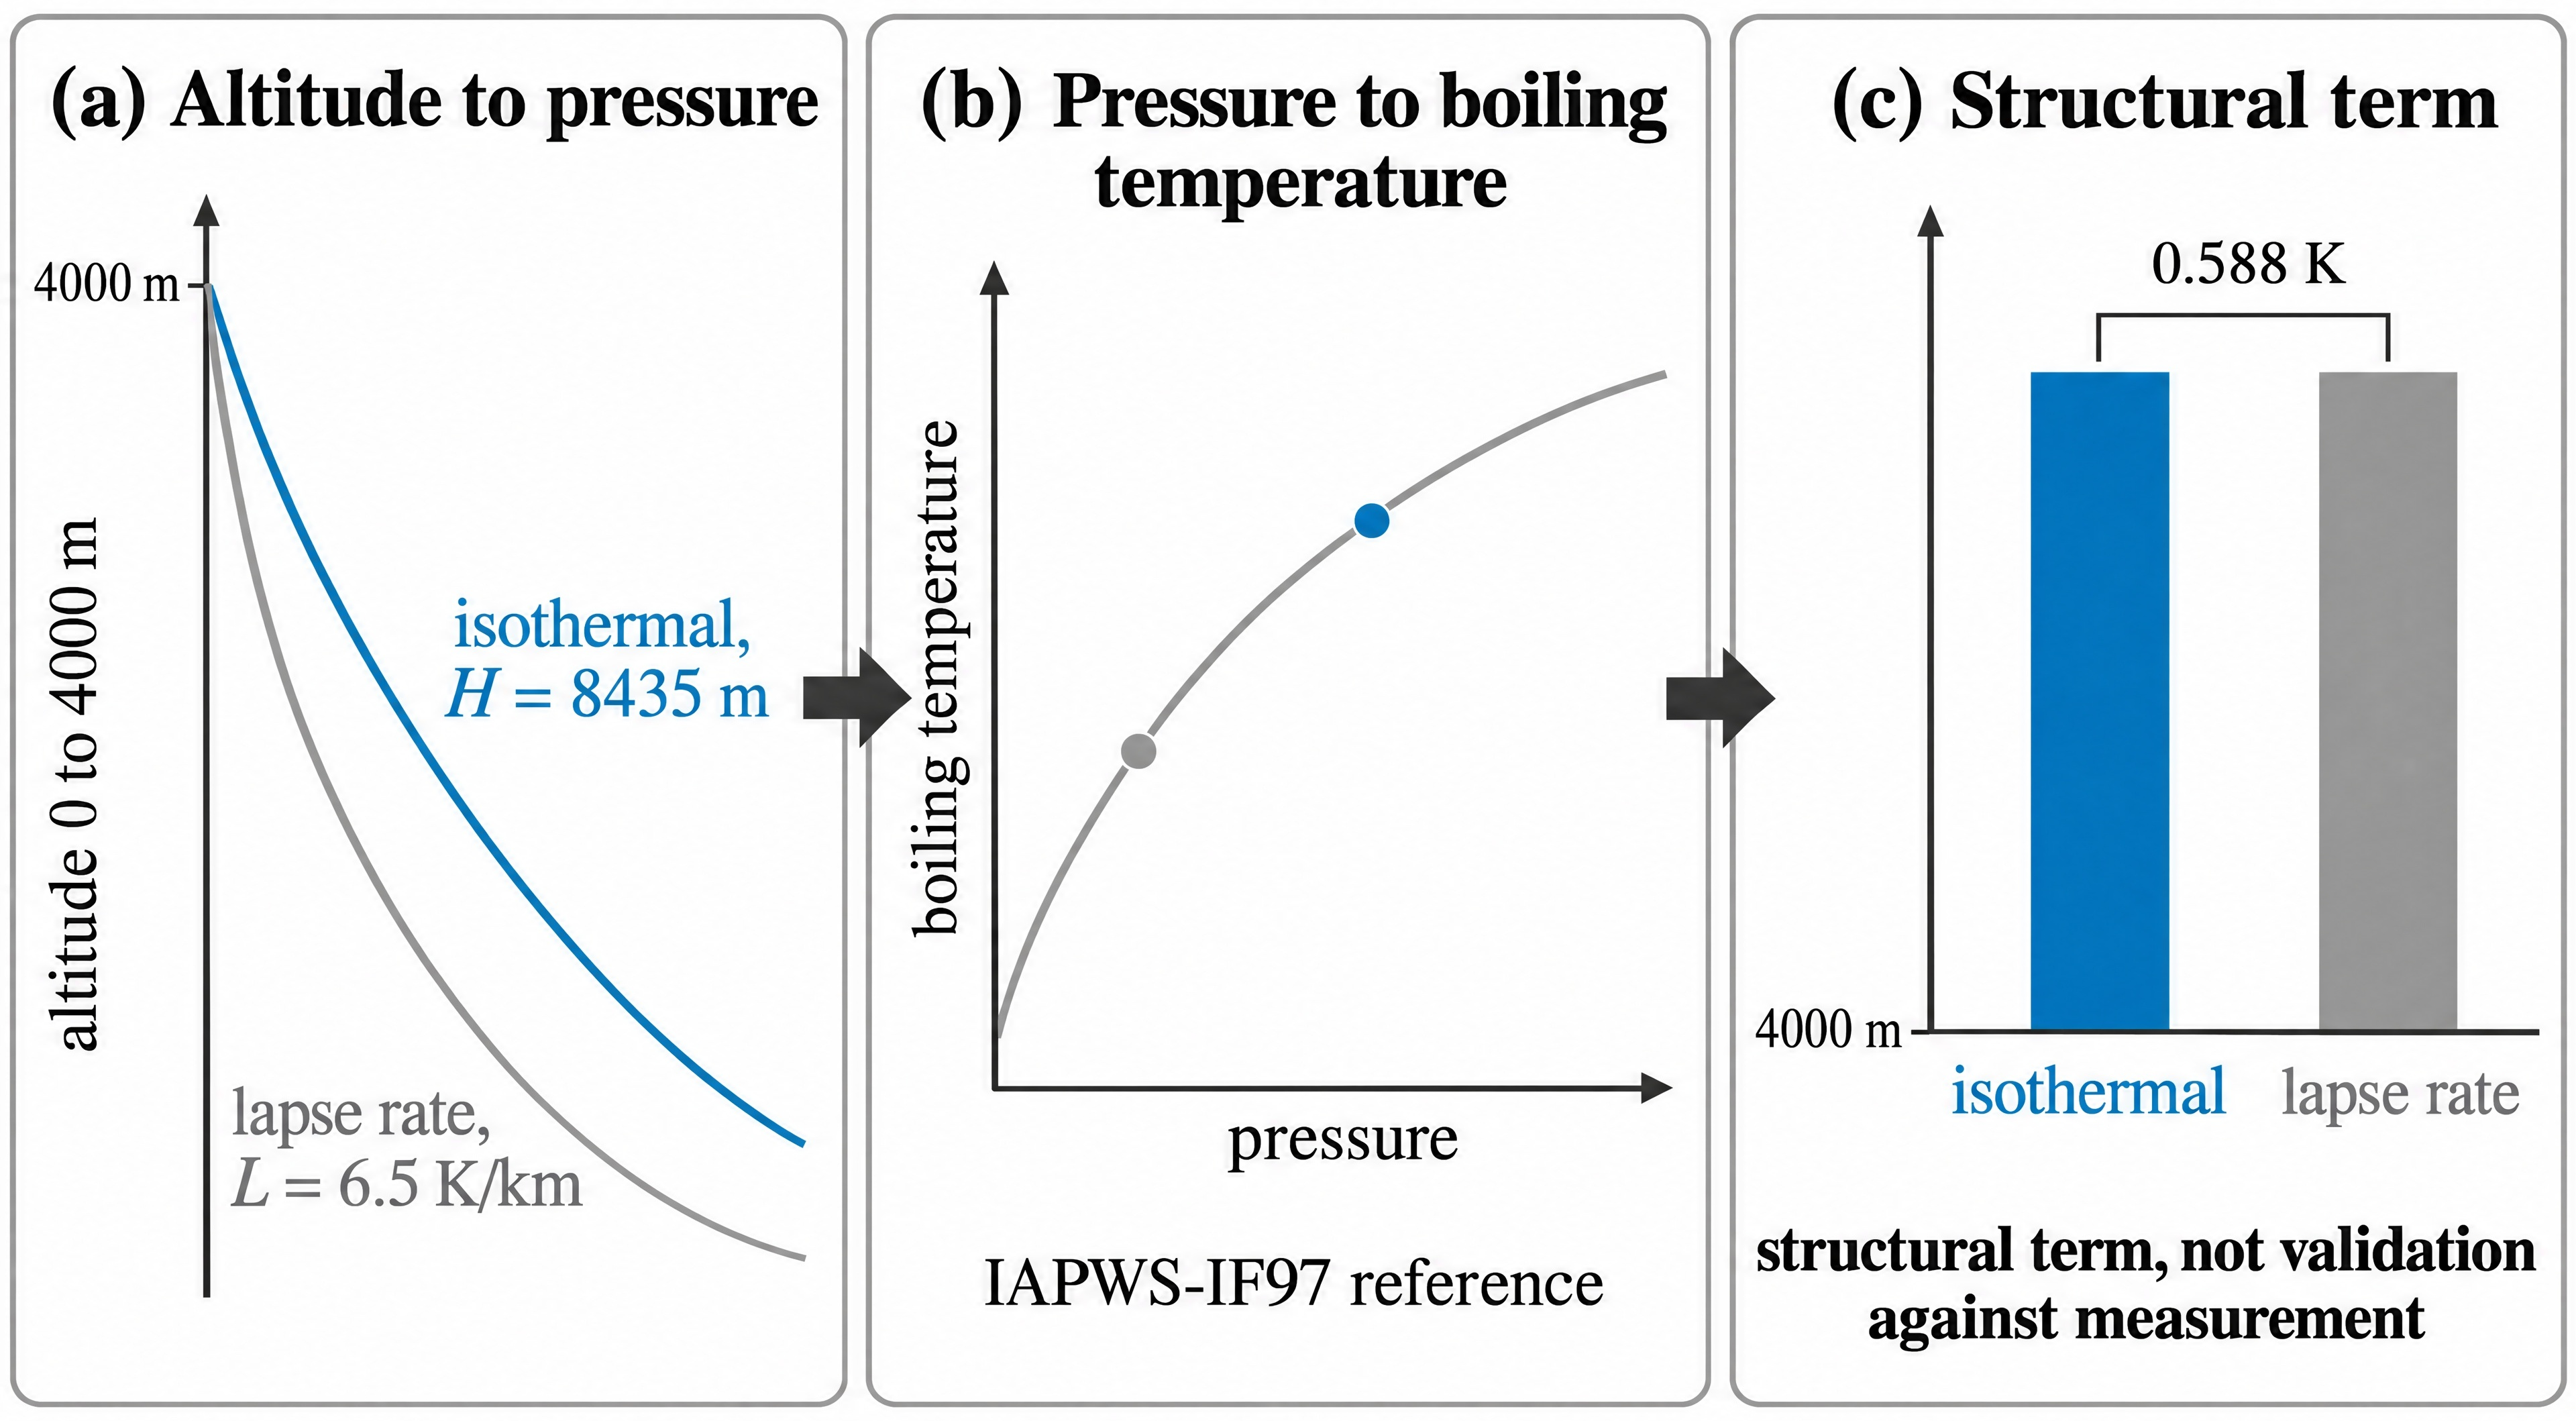
\includegraphics[width=\linewidth,height=0.45\textheight,keepaspectratio]{figures/fig1_v0.jpg}
  \caption{How a barometric boiling estimate is checked: an altitude feeds two pressure models, each pressure is inverted to a boiling temperature on the reference saturation curve, and their difference is the structural term, 0.588 K at 4000 m. This is a model-to-reference comparison, not validation against measurement. Blue marks the isothermal model, grey the lapse-rate model.}
  \label{fig:fig1}
\end{figure}

\begin{figure}[!htbp]
  \centering
  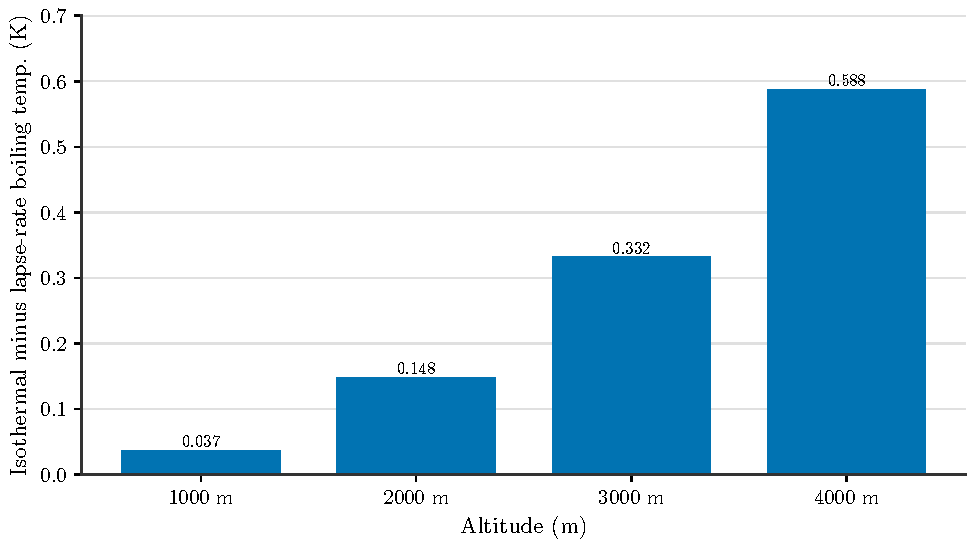
\includegraphics[width=\linewidth,height=0.45\textheight,keepaspectratio]{figures/fig2_v0.pdf}
  \caption{Model-only structural term, isothermal minus lapse-rate boiling temperature, at 1000--4000 m from the reference grid (exploratory; no measured data). The term grows from 0.037 K to 0.588 K and exceeds the 0.5 K structural target only between 3000 m (0.332 K) and 4000 m.}
  \label{fig:fig2}
\end{figure}

Section~\ref{sec:related} reviews the reference equations and the barometric models. Section~\ref{sec:method} gives the method. Section~\ref{sec:setup} describes the experimental setup, Section~\ref{sec:results} reports the results, and Sections~\ref{sec:discussion} and~\ref{sec:limitations} discuss the limits, before Section~\ref{sec:conclusion} concludes.

\section{Related Work}\label{sec:related}

\textbf{Reference saturation equations.} The IAPWS-95 Helmholtz equation of state for ordinary water and the IAPWS industrial formulation are the reference standards for water saturation properties. We use IAPWS-95 to invert saturation pressure to boiling temperature and region 4 of the IAPWS industrial formulation as the reference for the screen. Both are standards rather than measurements, so a match to them shows internal consistency, not agreement with laboratory boiling points. This is the same distinction the Introduction draws.

\textbf{Barometric pressure models.} The isothermal form assumes a single scale height. The lapse-rate form follows the troposphere temperature gradient of the U.S. Standard Atmosphere 1976, which we treat as the pressure reference. The difference between the two is the structural term that this paper measures. Models of the atmosphere ask what a pressure profile looks like; we ask what such a term does to a boiling temperature.

\textbf{Vapour-pressure routes.} Clausius-Clapeyron relations with constant or temperature-dependent latent heat, and empirical Antoine fits, are the routes most often used to turn pressure into boiling temperature. We compare these routes on one grid against one reference. We report held-out error, which an in-sample fit cannot show.

\section{Method}\label{sec:method}

We invert the saturation relation to find the boiling temperature $T_b$ at each ambient pressure $p$. The saturation pressure is given by the Wagner-Pruss (IAPWS-95) equation, and $T_b$ is found by bisection, with the inverse checked by round trip. The sea-level check gives $T_b = 373.1243$ K at $p = 101325$ Pa.

Two barometric pressure models supply $p$ as a function of altitude $z$. The isothermal model is $p_{\mathrm{iso}}(z) = p_0 \exp(-z/H)$, with scale height $H = 8434.5$ m. The lapse-rate model follows the troposphere relation $p_{\mathrm{lapse}}(z) = p_0 (1 - L z / T_0)^{g_0 / (R L)}$ with $L = 0.0065$ K/m, $T_0 = 288.15$ K, $p_0 = 101325$ Pa and $g_0 = 9.80665$ m/s$^2$. Its nodes match the tabulated Standard Atmosphere values to within 0.01 percent.

The structural term is $s(z) = T_{b,\mathrm{iso}}(z) - T_{b,\mathrm{lapse}}(z)$. Because the lapse-rate form reproduces the standard atmosphere, the structural term is the error the isothermal form adds to a boiling estimate. It is independent of the saturation equation, which cancels in the difference.

For the vapour-pressure routes, we compare three closed-form inversions on a 50 m grid from 0 to 4000 m: constant-latent-heat Clausius-Clapeyron, temperature-dependent-latent-heat Clausius-Clapeyron integrated from the normal boiling point with enthalpies from the IAPWS industrial formulation, and a three-parameter Antoine equation. The Antoine constants are fitted to the reference saturation curve on 273.15 to 363.15 K, and points from 363.15 to 373.15 K are held out. Pressure on the grid is the Standard Atmosphere pressure.

\section{Experimental Setup}\label{sec:setup}

The reference is the IAPWS industrial formulation saturation curve taken through the iapws package~\citep{iapws}, version 1.5.5, checked at the triple point (611.657 Pa) and at the normal boiling point (101325 Pa, within 5 Pa). No measured boiling records enter the reference.

For the structural term, we evaluate both barometric models on the shared reference grid at 100 m steps from 0 to 4000 m and report values at 1000, 2000, 3000 and 4000 m. The headline is tested against the 0.5 K structural target, which was fixed before the calculation. For the route comparison, we use 81 grid points from 0 to 4000 m, with the Antoine fit scored on 60 held-out points at 0 to 2950 m. Metrics are maximum absolute error, RMS error, bias, the altitude of the maximum, and the error at 4000 m. The 0.6 K total error bound is a budget for measured residuals and is not tested here.

The measured comparison was specified as follows. A measured record needs station pressure, elevation, observed boiling temperature and thermometer uncertainty. Accepted sites would be split into fit and holdout sets, with at least 15 accepted sites for a claim. We ran eight broad web queries, followed the most promising pages, and searched one dataset hub. Zero records met all four criteria.

\textbf{Code availability.} Code, prompts, raw outputs and the scripts that recompute each number are in the paper's code repository~\href{https://github.com/ai-inventor-papers/ai-invention-afc680-barometric-formula-predicts-waters/tree/main}{[code]}, and Appendix~\ref{app:code} links each result to the folder that produced it.

\section{Results}\label{sec:results}

\subsection{Structural term at 4000 m}\label{sec:headline}

On the shared reference grid (0 to 4,000 m), the isothermal form's structural term is 0.588 K at 4,000 m. That is 0.088 K above the 0.5 K structural target, so the target is missed. The result is a single exploratory, reference-only screen. It carries no interval, and it contains no measured data. An independent re-derivation reproduces the values at 3000 m and 4000 m. Figure~\ref{fig:fig2} shows the term at four altitudes against the target.

The term grows with altitude: 0.037 K at 1000 m, 0.148 K at 2000 m, 0.332 K at 3000 m and 0.588 K at 4000 m. It is a property of the model, so it holds whether or not the measured comparison is ever run.

\subsection{Vapour-pressure routes}\label{sec:routes}

Table~\ref{tab:routes} gives the held-out errors of the three routes against the reference, and Figure~\ref{fig:fig3} plots the same held-out RMS and maximum errors. On the 60 held-out points, the refitted Antoine equation has the lowest RMS error (0.061 K), ahead of temperature-dependent-latent-heat Clausius-Clapeyron (0.083 K) and constant-latent-heat Clausius-Clapeyron (0.108 K). On the full grid, constant-latent-heat Clausius-Clapeyron reaches 0.280 K at 4000 m, and temperature-dependent latent heat reaches 0.176 K at 4000 m. These are reference-only, exploratory estimates.

\begin{table}[!htbp]
  \centering
  \begin{tabular}{p{0.42\linewidth}p{0.15\linewidth}p{0.15\linewidth}p{0.18\linewidth}}
    \toprule
    Route & Held-out RMS (K) & Held-out max (K) & Altitude of held-out max (m) \\
    \midrule
    Constant-latent-heat Clausius-Clapeyron & 0.108 & 0.194 & 2950 \\
    Temperature-dependent-latent-heat Clausius-Clapeyron & 0.083 & 0.137 & 2950 \\
    Antoine refit (273.15 to 363.15 K) & 0.061 & 0.086 & 0 \\
    \bottomrule
  \end{tabular}
  \caption{Held-out errors against the IAPWS industrial formulation reference, 60 points at 0 to 2950 m.}
  \label{tab:routes}
\end{table}

\begin{figure}[!htbp]
  \centering
  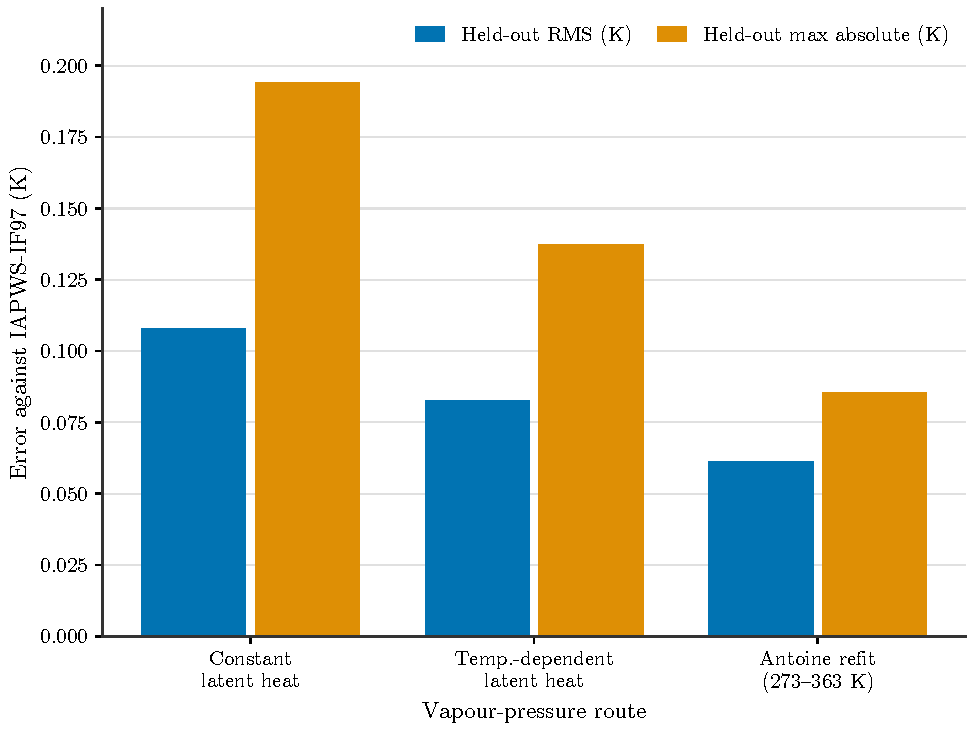
\includegraphics[width=\linewidth,height=0.45\textheight,keepaspectratio]{figures/fig3_v0.pdf}
  \caption{Held-out RMS and maximum absolute error of three vapour-pressure routes against the IAPWS industrial formulation reference, over 60 grid points at 0--2950 m. The constant and temperature-dependent latent-heat forms are Clausius--Clapeyron routes. The Antoine refit has the lowest error on both measures, but this is exploratory and provisional.}
  \label{fig:fig3}
\end{figure}

The Antoine ranking is provisional. An in-sample RMS for the refit (0.0042 K) could not be reproduced, and repeating that fit gives 0.036 K. A sensitivity fit on 273.15 to 353.15 K changes the held-out error by 0.03 K. The ranking therefore depends on the fit range. The Clapeyron relation holds once the ideal-vapour assumption is corrected by the vapour compressibility factor: the residual falls from 1.63 percent to 0.06 percent. That check is close to an identity, because the same equations supply its inputs. An independent IAPWS-95 derivative check gives 0.06 percent.

\subsection{Measured comparison}\label{sec:measured}

No measured record was accepted, so the comparison with published boiling points is not testable. All three claims on the measured side are untested. The predicted-minus-observed residual, its holdout statistics and the verdict on the 0.6 K total bound are all absent.

\section{Discussion}\label{sec:discussion}

The structural term is the part of the boiling error that a reader can compute without any measurement. At 2000 m it is 0.148 K, and whether that is practically negligible depends on the measurement uncertainty, which this run could not establish. The term crosses the 0.5 K target between 3000 m and 4000 m, and at 4000 m it is 0.588 K. A user who needs a boiling estimate at that height should not rely on the isothermal form without a measurement.

The route comparison says more about fit range than about physics. A fit that is judged on held-out points can rank routes differently from one judged on its own training points, and in this run the ranking changed with the fit range. An evaluation of a boiling formula should therefore report held-out error and the fit range together.

\section{Limitations}\label{sec:limitations}

The central limitation is that no measured boiling record was verified. The paper therefore answers how the barometric formula departs from a reference equation, not how it departs from measured boiling points, which is the question asked. The measured comparison needs records with station pressure, elevation, observed boiling temperature and thermometer uncertainty, and a fixed holdout set. None of these exist in our data.

The headline is a single screen on one shared reference grid, with no interval. It was not registered in advance as a test, and its 0.5 K target is a structural threshold, not a measured tolerance.

The structural term is computed on one reference pressure model. Our lapse-rate form follows the Standard Atmosphere 1976 troposphere, and the primary standard document was not read directly. Its values agree with the tabulated nodes, so the effect on the result is small, but the provenance is secondary.

The Antoine ranking is provisional. It depends on fit range, and the in-sample value obtained in one run did not reproduce on repetition. The Clapeyron check is largely an identity, because the same reference equations supply its inputs. The 0.6 K total bound is untested.

Finally, the study covers one altitude range, 0 to 4000 m, and one water-only chemistry. Humidity, weather-driven pressure changes and dissolved solutes are excluded.

\section{Conclusion}\label{sec:conclusion}

On the shared reference grid, the isothermal barometric formula adds a structural error to a boiling estimate that grows with altitude, reaching 0.588 K at 4,000 m, 0.088 K above the 0.5 K structural target. This is a single exploratory, reference-only screen with no interval. Whether the formula agrees with measured boiling points within the 0.6 K total budget cannot be said from this work. Measured records with station pressure, elevation and thermometer uncertainty are needed to answer the question asked, and the held-out comparison of vapour-pressure routes should be repeated on them.

\clearpage
\bibliographystyle{plainnat}
\bibliography{references}

\clearpage
\appendix
\section{Code for each result}\label{app:code}

Each row below links the code folder, on the run's code branch, of the experiment behind a result.

\begin{longtable}{p{0.2\linewidth}p{0.36\linewidth}p{0.36\linewidth}}
  \toprule
  Section & Result & Code folder \\
  \midrule
  \endhead
  \S\ref{sec:intro} & Structural term at 4000 m (headline, Figure~\ref{fig:fig2}) & \href{https://github.com/ai-inventor-papers/ai-invention-afc680-barometric-formula-predicts-waters/tree/main/round-1/experiment-1}{\texttt{round-1/experiment-1}} \\
  \S\ref{sec:headline} & Structural term at 4000 m (Figure~\ref{fig:fig2}) & \href{https://github.com/ai-inventor-papers/ai-invention-afc680-barometric-formula-predicts-waters/tree/main/round-1/experiment-1}{\texttt{round-1/experiment-1}} \\
  \S\ref{sec:intro} & Vapour-pressure route comparison (Table~\ref{tab:routes}, Figure~\ref{fig:fig3}) & \href{https://github.com/ai-inventor-papers/ai-invention-afc680-barometric-formula-predicts-waters/tree/main/round-2/experiment-4}{\texttt{round-2/experiment-4}} \\
  \S\ref{sec:routes} & Vapour-pressure route comparison (Table~\ref{tab:routes}, Figure~\ref{fig:fig3}) & \href{https://github.com/ai-inventor-papers/ai-invention-afc680-barometric-formula-predicts-waters/tree/main/round-2/experiment-4}{\texttt{round-2/experiment-4}} \\
  \S\ref{sec:intro} & Measured comparison (no accepted records; all claims untested) & \href{https://github.com/ai-inventor-papers/ai-invention-afc680-barometric-formula-predicts-waters/tree/main/round-2/experiment-3}{\texttt{round-2/experiment-3}} \\
  \S\ref{sec:measured} & Measured comparison (no accepted records; all claims untested) & \href{https://github.com/ai-inventor-papers/ai-invention-afc680-barometric-formula-predicts-waters/tree/main/round-2/experiment-3}{\texttt{round-2/experiment-3}} \\
  \bottomrule
\end{longtable}

\end{document}
